%%%%%%%%%%%%%%%%%%%%%%%%%%%%%%%%%%%%%%%%%%%%%%%%%%%%%%%%%%%%%%%%%%%%%
%% This is a (brief) model paper using the achemso class
%% The document class accepts keyval options, which should include
%% the target journal and optionally the manuscript type. 
%%%%%%%%%%%%%%%%%%%%%%%%%%%%%%%%%%%%%%%%%%%%%%%%%%%%%%%%%%%%%%%%%%%%%

% Langd5 es el template para LANGMUIR
\documentclass[journal=langd5,manuscript=article]{achemso}

%%%%%%%%%%%%%%%%%%%%%%%%%%%%%%%%%%%%%%%%%%%%%%%%%%%%%%%%%%%%%%%%%%%%%
%% Place any additional packages needed here.  Only include packages
%% which are essential, to avoid problems later. Do NOT use any
%% packages which require e-TeX (for example etoolbox): the e-TeX
%% extensions are not currently available on the ACS conversion
%% servers.
%%%%%%%%%%%%%%%%%%%%%%%%%%%%%%%%%%%%%%%%%%%%%%%%%%%%%%%%%%%%%%%%%%%%%
\usepackage[version=3]{mhchem} % Formula subscripts using \ce{}

%%%%%%%%%%%%%%%%%%%%%%%%%%%%%%%%%%%%%%%%%%%%%%%%%%%%%%%%%%%%%%%%%%%%%
%% If issues arise when submitting your manuscript, you may want to
%% un-comment the next line.  This provides information on the
%% version of every file you have used.
%%%%%%%%%%%%%%%%%%%%%%%%%%%%%%%%%%%%%%%%%%%%%%%%%%%%%%%%%%%%%%%%%%%%%
%%\listfiles

%%%%%%%%%%%%%%%%%%%%%%%%%%%%%%%%%%%%%%%%%%%%%%%%%%%%%%%%%%%%%%%%%%%%%
%% Place any additional macros here.  Please use \newcommand* where
%% possible, and avoid layout-changing macros (which are not used
%% when typesetting).
%%%%%%%%%%%%%%%%%%%%%%%%%%%%%%%%%%%%%%%%%%%%%%%%%%%%%%%%%%%%%%%%%%%%%
\newcommand*\mycommand[1]{\texttt{\emph{#1}}}

%%%%%%%%%%%%%%%%%%%%%%%%%%%%%%%%%%%%%%%%%%%%%%%%%%%%%%%%%%%%%%%%%%%%%
%% Meta-data block
%% ---------------
%% Each author should be given as a separate \author command.
%%
%% Corresponding authors should have an e-mail given after the author
%% name as an \email command. Phone and fax numbers can be given
%% using \phone and \fax, respectively; this information is optional.
%%
%% The affiliation of authors is given after the authors; each
%% \affiliation command applies to all preceding authors not already
%% assigned an affiliation.
%%
%% The affiliation takes an option argument for the short name.  This
%% will typically be something like "University of Somewhere".
%%
%% The \altaffiliation macro should be used for new address, etc.
%% On the other hand, \alsoaffiliation is used on a per author basis
%% when authors are associated with multiple institutions.
%%%%%%%%%%%%%%%%%%%%%%%%%%%%%%%%%%%%%%%%%%%%%%%%%%%%%%%%%%%%%%%%%%%%%
\author{Mar\'ia Laura V\'azquez Juiz}
\affiliation[UVIGO Campus Auga]{Facultad de Ciencias, Campus da Auga, University of Vigo}

\author{Diego Soto G\'omez}
\email{disoto@uvigo.es}
\affiliation[UVIGO Campus Auga]{Facultad de Ciencias, Campus da Auga, University of Vigo}

\author{Paula P\'erez Rodr\'iguez}
\affiliation{Instituto Nacional de Investigaciones Agrarias,
Carretera de La Coru\~na km 7,5 Madrid}
\alsoaffiliation{Facultad de Ciencias, Campus da Auga, University of Vigo}

\author{Marcos Paradelo P\'erez}
\email{marcos.paradelo@agro.au.dk}
\affiliation{Department of Agroecology, University of Aarhus}
\alsoaffiliation{Facultad de Ciencias, Campus da Auga, University of Vigo}

\author{Jos\'e Eugenio L\'opez Periago}
\affiliation[UVIGO Campus Auga]{Hydraulics Lab,Faculty of Sciences, Campus da Auga, University of Vigo}
\altaffiliation{Current address:  Edificio polit\'ecnico s/n As Lagoas 32004 Ourense, Spain}
%\email{edelperi@uvigo.es}
\phone{+34 (9)88 387070}
\fax{+34 (9)88 387001}


\title[Resolving particle size in polydisperse mixtures by TRPS]
  {Resolving the particle size distribution in polydisperse polystyrene latex
  microspheres-humic acid mixtures using Tunable Resistive Pulse
  Sensing\footnote{Resolving particle distribution in polidisperse
  suspensions using TRPS}}

%%%%%%%%%%%%%%%%%%%%%%%%%%%%%%%%%%%%%%%%%%%%%%%%%%%%%%%%%%%%%%%%%%%%%
%% Some journals require a list of abbreviations or keywords to be
%% supplied. These should be set up here, and will be printed after
%% the title and author information, if needed.
%%%%%%%%%%%%%%%%%%%%%%%%%%%%%%%%%%%%%%%%%%%%%%%%%%%%%%%%%%%%%%%%%%%%%
\abbreviations{BIC,DLVO,HA,MS,PBE,PSD,TRPS}
\keywords{Bayesian Information Criteria, Clustering, Humic Acid, Dejarguin-Landau-Vervey-Oberbeek,Polystyrene-latex Microspheres,Particle Balance Equation,Particle Size Distribution,Tunable Resistive Pulse Scanning}

%%%%%%%%%%%%%%%%%%%%%%%%%%%%%%%%%%%%%%%%%%%%%%%%%%%%%%%%%%%%%%%%%%%%%
%% The manuscript does not need to include \maketitle, which is
%% executed automatically.
%%%%%%%%%%%%%%%%%%%%%%%%%%%%%%%%%%%%%%%%%%%%%%%%%%%%%%%%%%%%%%%%%%%%%
\begin{document}

\tableofcontents
%%%%%%%%%%%%%%%%%%%%%%%%%%%%%%%%%%%%%%%%%%%%%%%%%%%%%%%%%%%%%%%%%%%%%
%% The "tocentry" environment can be used to create an entry for the
%% graphical table of contents. It is given here as some journals
%% require that it is printed as part of the abstract page. It will
%% be automatically moved as appropriate.
%%%%%%%%%%%%%%%%%%%%%%%%%%%%%%%%%%%%%%%%%%%%%%%%%%%%%%%%%%%%%%%%%%%%%
\begin{tocentry}

%Some journals require a graphical entry for the Table of Contents.
%This should be laid out ``print ready'' so that the sizing of the
%text is correct.




\end{tocentry}

%%%%%%%%%%%%%%%%%%%%%%%%%%%%%%%%%%%%%%%%%%%%%%%%%%%%%%%%%%%%%%%%%%%%%
%% The abstract environment will automatically gobble the contents
%% if an abstract is not used by the target journal.
%%%%%%%%%%%%%%%%%%%%%%%%%%%%%%%%%%%%%%%%%%%%%%%%%%%%%%%%%%%%%%%%%%%%%
\begin{abstract}



Size and polydispersivity have an enormous influence on 
colloid transport in natural porous media and packed filters.
Coating of colloidal particles by natural polymers  adds complexity. 

Several techniques Light scattering has an intrinsic difficulty to resolve the particle size in polydisperse colloidal suspensions.
Tunable Resistive Pulse Scanning TRPS is new technique based on the Coulter principle that measures the particle size individually. This feature can be used to resolve the components of mixed sizes distributions in polydisperse aqueous suspensions.


In this work used TRPS and statistical clustering to resolve the components of a mixture of particle sizes in the range 
from $500$ to $2000~\mathrm{nm}$. 

These advantages were used to examine the coating of polystyrene by Humic Acids cation, polymer bridging and polymer stabilization.






\end{abstract}


%%%%%%%%%%%%%%%%%%%%%%%%%%%%%%%%%%%%%%%%%%%%%%%%%%%%%%%%%%%%%%%%%%%%%
%% Start the main part of the manuscript here.
%%%%%%%%%%%%%%%%%%%%%%%%%%%%%%%%%%%%%%%%%%%%%%%%%%%%%%%%%%%%%%%%%%%%%
\section{Introduction}

%Importancia de la distribución de tamaños de los coloides.

The most importance factor on the retention of colloid in porous media is the
particle size. Particle size distribution PSD has an enormous importance on the
behavior of substances in environment.
%Introducir citas y ejemplos.

%=========================================================================
%Aplicaciones 
Understanding  the role of the soil humic polymers on the colloid behavior of
natural and engineered particles in soil and porous media in general  may contribute to further technical developments based in the control of colloidal processes in fields related to 
water quality, environment, and public health~\cite{Ngo2008}
\cite{Farre2011}

Presence of HA and FA have a remarkable influence on the removal of metal contaminants 
\ce{Cr(VI)}  
and
\ce{As(V)} 
by zero-valent Fe nanoparticles~\cite{Mak2011234}.


%=========================================================================

%% El problema de determinación de tamaños en suspensiones de tamaños coloidales polidispersos

Dynamic light scattering (DLS)  cannot resolve variation in size as the scattering angle is increased through minima in the intensity form factor.
Some efforts have been made to characterize of the particle size distributions of colloidal particles with small polydispersities using a combination of DLS and static light scattering and two-color laser sources to avoid contributions from multiple scattering. However the results cannot discriminate different particle populations~\cite{Bryant2003AccurateSuspensions}. These authors report heavy tailed distributions but they do not report population mixtures.




\subsection{Polymer coating and colloid behavior}

%importancia de la cubierta polimérica y que efectos  tiene sobre el comportamiento de l.os coloides
Polymer coating by dissolved polymers affect dramatically the mobility of colloid-size particles in the aqueous environments.
For example, the retention of pathogenic microorganisms~\cite{Morales2011a}, ie., the travel distances along  subsurface environments, depends largely on characteristics of the polymer coating, cross linking can favor the coagulation,bridging flocculation,which enhances the colloid retention by several orders of magnitude. Conversely,  stabilization by adsorbed polymers can enhance transport.

The particle size effect dominated over the flow rate and organic matter polymer can block the adsorption sites in sand filters~\cite{Yang2015InterplayModeling}.

Conformation of polymers attached to particle surfaces is controlled by the cover density, pH and ions. These determine the polymer coiling. Therefore the size can of suspended colloids vary upon the electrochemical environment~\cite{Morales2011a}


Study of polymeric coating   on surfaces can be cumbersome,
~\citeauthor{doi:10.1021/es981236u}\cite{doi:10.1021/es981236u}
used  \ce{Si/SiO2} wafer strips  a coated with  polystyrene as support for
adsorption studies of HA laser-beam reflectometry. That procedure is
limited by technique of coating flat surfaces with a desired compound so, to date, that cannot be used with  natural colloids or microorganisms.

%Tamaño de los HA (esto puede ir a métodos) de momento no lo  ponemos
%Size of humic acid can be measured by several (electron microscopy, light scattering, size exclusion chromatography).  

%Basic structure and size of soil humic acids from a Dystric Cambisol (WRF) by small-angle X-ray scattering, and small-angle neutron scattering in $50~\mathrm{mM}$ \ce{NaOH\; Na2B3O7} buffer \ce{pH\, 10} was reported ~\cite{Kawahigashi1995}. They reported a core of high electron
%density with a radius of 
%$3.0~\mathrm{nm}$
%surrounded by branches with a radius of gyration between 
%$5.8$ to $7.5~\mathrm{nm}$.





% Métodos disponibles para deteminar el tamaño de los coloides.
%\subsection{State of art on methods to determine  the particle size}





\subsection{Particle size}
% En que consiste el TRPS
TRPS method uses the same
principle of the Coulter method. It
calculates the size of individual particles 
and determines the  concentration of particles in the sample.
%Ventajas del TRPS 

TRPS has enough resolution to discriminate populations mixed in multimodal
samples polystyrene bead~\cite{Varenne2016MultimodalMethods}. 
In adition, TRPS does not disturb the geometry of the particle, such as  the
TEM or SEM, which need to dry the suspension before measurement.
%inconvenientes
One drawback of this technique is that electric conductivity of the buffer
used in TRPS.
Electrolyte must met the requirements of current intensity and
voltage for accurate measurements of the blockades.
Since the most of the applications have been developed to 
biological fluids, and buffers typically used in cellular biology  such as PBS or Tris.
This constitutes an
important limitation in the span of  experimental conditions  required in the  earth surface environment, i.e. surface and subsurface waters, with a larger  span of \ce{pH} and electrolyte composition.
Therefore, a setup of electrolyte 


%
Another limitation is the representativity of the sample. Size is determined in a very small sample of particles, about  $500$ counts in samples with $10^9$ particles per liter.



%Por hacer:
%Eugenio .- Efectos de ángulo de trayectoria de las MS sonbre los blockades.
% Produce distribuciones con dos picos, el segundo está asociado a trayectorias con ángulos cerrados.\cite{Weatherall2016}

%========================================================================
%Objectives
%========================================================================
The objective of this work was testing the capabilities of TRPS to identify
particle size mixtures in  polydisperse colloid suspensions.

In a primary approach the TRPS was used to examine the HA coating of
polystyrene latex beads by measuring the changes of the particle size
distribution.


%%%%%%%%%%%%%%%%%%%%%%%%%%%%%%%%%%%%%%%%%%%%%%%%%%%%%%%%%%%%%%%%%%%%%
%% Theory
%%%%%%%%%%%%%%%%%%%%%%%%%%%%%%%%%%%%%%%%%%%%%%%%%%%%%%%%%%%%%%%%%%%%%
%\section{Theory}
%teoría de la formación de recubriemientos poliméricos sobre partículas coloidales
% Gregory, Elimelech


%%%%%%%%%%%%%%%%%%%%%%%%%%%%%%%%%%%%%%%%%%%%%%%%%%%%%%%%%%%%%%%%%%%%%
%% Experimental
%%%%%%%%%%%%%%%%%%%%%%%%%%%%%%%%%%%%%%%%%%%%%%%%%%%%%%%%%%%%%%%%%%%%%
\section{Experimental} % Langmuir
%\section{Materials and methods} %ES&T
%Laura:
\subsection{Particle size measurement}
%Laura:
We used a NP1000 nanopore that measures sizes between 500 and
$2000~\mathrm{nm}$.
This interval is optimal for measuring the
$1000~\mathrm{nm}$ 
microspheres used in this study.


All buffer and electrolytes used in the particle size measurements were
prepared withultrapure water
Milli-Q (Millipore-Merk)  filtered through a membrane
$< 220~\mathrm{nm}$).

%buffers
Concentrations of  \ce{NaCl} and \ce{CaCl2} were optimized to reach the 
same operational conditions of measurement used in the
calibration with the microspheres used as standards in
phosphate saline buffer (PBS,
\ce{Cl2H3K2Na3O8P2}).
The optimal concentrations, pH and the ionic strength of the buffers are shown in Table~\ref{tbl:electrolytes}. 

%!!!!!!!!!!!!!!!!!!!!!!!!!!!!!!!!!!!!!!!!!!!!!
%  LAURA:     FALTAN LOS PH!!!!
\begin{table}
\caption{Characteristics of the electrolytes used in the TRPS measurements}
\label{tbl:electrolytes}
  \begin{tabular}{lrrr}
Electrolyte & Conc. & \ce{pH}  & $I$ \\
\hline
PBS &	152 & ????	&	172 \\
\ce{NaCl} &	14	& 	???? &	14\\
\ce{CaCl2} &	7	& ???? &	21\\
\hline
\multicolumn{4}{p{0.4\linewidth}}{
Conc., concentration $\mathrm{mmol\,L^{-1}}$; 
$I$, ionic strength  $\mathrm{mmol\,L^{-1}}$; 
}
\end{tabular}
\end{table}
%!!!!!!!!!!!!!!!!!!!!!!!!!!!!!!!!!!!!!!!!!!!!!

%Colloids
The colloid suspensions used in the experiments were latex microspheres (MS), humic acids (HA) and mixtures of microspheres and humic acids (MS-HA).

%polystyrene
Polystyrene latex MS,
Estapor Merck-Millipore, Darmstadt Germany, Ref. F-Y 100, Lot number 953 B1,
had a mean diameter of $930 \, \pm 10~\mathrm{nm}$ 
without surface functional groups.
The stock suspension had a polystyrene concentration of $10~\mathrm{g\,L^{-1}}$.

Humic acids were purchased from from Merck-Sigma-Aldrich,
humic acid sodium salt technical grade CAS Number 68131-04-4,
with a molecular weight range of 2,000--500,000.
 A stock suspension was prepared by dissolving 
$\mathrm{0.1\,g}$ HA in $100~\mathrm{mL}$ ultrapure water.

The mixture was prepared with different concentrations of humic acids to know if covering was produced. The MS suspension was a dilution 1:1000 from the stock. 


%Laura:Measurements in the TRPS: buffer (less than a minute), buffer + HA (3 minutes approximately) and buffer + MS + HA (lasted a minimum of 30 seconds). 

%Measurement protocol in the TRPS


All the suspensions were prepared in three buffers: \ce{CaCl2},
PBS and \ce{NaCl}. 
All the suspensions were vortexed 
and filtered just before injecting in the TRPS apparatus.

%!!!!!!!!!!!!!!!!!!!!!!!!!!!!!!!!!!!!!!!!!!!!!!!!!!!
%Eugenio: cuanto volumen de buffer pusiste en cada parte de la célula del TRPS? 40 uL?
$\mathrm{40 \,\mu L}$ buffer
was put in the lower
fluid cell and in the upper fluid cell. The parameters were
adjusted to a current with values between 70 and 150 nA. Once
the current was stable, the samples were injected in the upper cell.
The experimental conditions chosen for the three buffers  were identical, with a pore stretch of $47~\mathrm{mm}$.
The total pressure different between the two halves of the fluid cell was 
$66~\mathrm{Pa}$, 
the sames used by other authors~\cite{Weatherall2016}.
The voltages were 
$0.08~\mathrm{V}$ for PBS, and 
$0.7~\mathrm{V}$ for both
\ce{NaCl} and
\ce{CaCl2}. 


		

% Pressure & Inherent p./ Pa & Inherent p./ cm H2O  & Actual pressure/ Pa & Actual pressure/ cm H2O \\
%\hline
% 20 & 46 & 0.47 & 66 & 0.674347826\\


The device measurement thresholds are 30 seconds minimum
and 10 minutes the maximum time for the measurement to be
optimal, provided that a minimum of 500 blockades is reached
for the 30 seconds case.



%Experimental plan

Influence of concentration of HA and contact time on the size  distribution of MS were evaluated.
Five concentrations of HA, namely 
2, 4, 6, 8 and  10 $\mathrm{mg\,L^{-1}}$
and a control of MS without HA
were incubated for 
0.25, 16 y 41 h in 
%14 mM \ce{NaCl} and
7 mM\ce{CaCl2}
%, pH  ???????
.
All experiments were made in triplicate.





%=================== End of the experimental section ==========



\subsection{Particle size clustering}




Analysis of particle size populations was done by    
a model-based clustering, classification, and density estimation based on
finite Gaussian mixture modeling.  The clustering model used is the 
expectation-maximization (EM) algorithm, a general description can be read in 
\citeauthor{Do2008}  
\citeyear{Do2008}
\cite{Do2008}.  

Briefly, each population of a finite  mixture density is usually associated with a group or cluster. In this work we assume that all component densities arise from the same parametric distribution family. The model assumes a univariate Gaussian distribution for each component or cluster. In one dimension, there are just two models, all component have equal variance or varying variance among components.
The model selection was based on the Bayesian Information Criteria (BIC).
Details about the clustering procedure and information of the mclust library used for calculations can be read in 
~\citeauthor{Fraley2012MclustEstimation}\cite{Fraley2012MclustEstimation}. The mclust library is implemented in the R statistical package~\cite{RCoreTeam2011}.





%%%%%%%%%%%%%%%%%%%%%%%%%%%%%%%%%%%%%%%%%%%%%%%%%%%%%%%%%%%%%%%%%%%%%
%% Results
%%%%%%%%%%%%%%%%%%%%%%%%%%%%%%%%%%%%%%%%%%%%%%%%%%%%%%%%%%%%%%%%%%%%%
\section{Results}
%\section{Results and discussion} %ES&T




%===========================================================
% En esta sección se describen los resultados de probar los
% buffers NaCl y CaCl2
\subsection{Buffers}
%-------------------------------------------------------------
  
  %Masa molecular NaCl 58.44 g/mol
  %Masa molecular CaCl_2  110,98 g/mol
  
  
%quedei
%PBS
%Molecular Formula: 	Cl2H3K2Na3O8P2
%Molecular Weight: 	411.029 g/mol
  
 %PBS 8,2 mol/l  3379,5 ppm
 
 
 
%LAURA que oncentraciones de MS utilizaste para las pruebas de HA y ? 
 %Resultado (revisar)


Optimal conditions of baseline current magnitude and  stability, and blockade readings  were obtained with 
 \ce{NaCl\; 5.5\,mmol\,L^{-1}}
 \ce{CaCl2\; 2.5\,mmol\,L^{-1}}.
 
 
 

 

%\begin{table}
%\label{tbl:control_baseline_blockades}
%\caption{Average blockade rate ,$\mathrm{nC\,s^{-2}}$, of MS
%and HA ($10~\mathrm{mg\,L^{-1}}$)
%in electrolyte (\ce{CaCl2} $\mathrm{7\, mmol\,L^{-1}}$). Control %is electrolyte only.
%}
%\begin{tabular}{
%l r@{$\pm$}l 
%r@{$\pm$}l
%}
%Test & \multicolumn{2}{c}{blockade rate} &nA 10 min\\
%\hline
%MS & 10.1 & 2.66 & 6057 \\
%HA  & 0.042  & 0.059 & 25\\
%Control & 0.008 & 0.007 & 5\\
%\hline
%\multicolumn{3}{p{0.3\linewidth}}{Control }
%\end{tabular}
%\end{table}


Comparison of 
blockade magnitude and duration 
for these electrolytes and the PBS buffer, used as standard, is shown in Figure~\ref{fgr:pairs_buffers}.
%%=============================================================
 \begin{figure}
  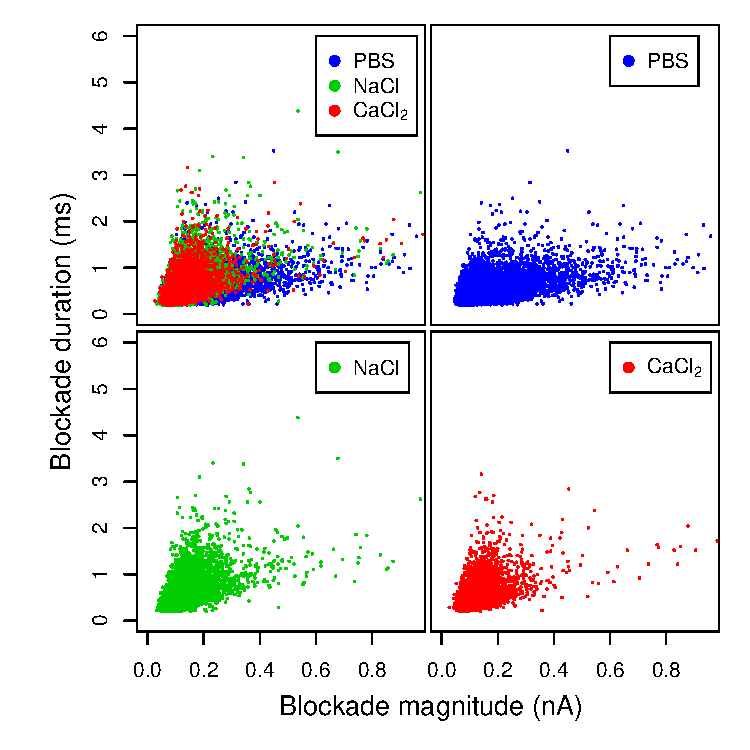
\includegraphics[width=\linewidth]{Figures/Pairs_buffers_MS.pdf}
  \caption{Scatter-plot comparing  blockade magnitude and blockade duration of  polystyrene microspheres for three electrolytes. The core of the point cloud is similar in the three elecrolytes. PBS  present the largest  disp/ersion in the blockade magnitude.} 
  \label{fgr:pairs_buffers}
\end{figure}
%% ===========================================================
Note that  the scattering patterns \ce{NaCl}  and \ce{CaCl2} are almost identical  similar, while PBS showed the largest  variation in the blockade magnitude.
Table~\ref{tbl:clustering_buffers} shows that the number of blockades was similar for the electrolytes and PBS.


  











\begin{table}
\label{tbl:clustering_buffers}
\caption{2D  clustering results of
 blockade magnitude and  duration 
 for three buffers
using the gaussian finite mixture model fitted by EM algorithm
}
\begin{tabular}{rrrrrrr}
& \multicolumn{2}{c}{\ce{CaCl2}} &
  \multicolumn{2}{c}{\ce{NaCl}} &
  \multicolumn{2}{c}{PBS} \\
\hline
\# & nblk & MP &
    nblk & MP &
    nblk & MP \\ 
\hline
1 & 13 &  0.004  & 1068 &   0.328 &  447 &    0.119 \\
2 & 587 & 0.137  & 988 &    0.283&   342 &    0.107 \\
3 & 1340 & 0.357 & 739 &    0.237&   787 &    0.206 \\
4 & 1332 & 0.343 & 231 &    0.077&   713 &    0.215 \\
5 & 331 & 0.106  & 174 &    0.062 &  80 &     0.019 \\
6 & 76 &  0.022  & 8 &      0.003 &  1059 &   0.291\\
7 & 72 &  0.032  & 18 &     0.009 &  54 &     0.017 \\
8 &    &         & 2 &      0.001 &  104 &    0.024 \\
\hline
Sum &3751 &&  3288  && 3586 &  \\   
\hline
\multicolumn{7}{p{0.5\linewidth}}{nblk number  of blockades in the cluster ;MP, mixing probabilities.}\\
\end{tabular}
\end{table}


% Testing the background blockades using buffers and HA
Electrolyte,
\ce{CaCl2} $\mathrm{2.5\, mmol\,L^{-1}}$
$\mathrm{pH}\,6$ 
gave about six blockades after $\mathrm{600\,s}$.
Blockade rate using the highest concentration of 
HA ($10~\mathrm{mg\,L^{-1}}$) in \ce{CaCl2}
 was $0.042\,\pm0.059~\mathrm{nA\,s^{-1}}$.
Blockade rate using the MS in \ce{CaCl2} 
was 240 times higher than HA. Therefore the contribution of  unbound HA to blockades in  HA-MS mixtures can be neglected, and
blockades can be assigned mostly to MS.


\subsection{HA-MS interaction}

%%==============================================================
\begin{table}
\caption{Double layer sphere-sphere interaction  of HA and MS using the standard DLVO calculations assuming constant potential.}
\label{tbl:dvlo_interaction}
\begin{tabular}{lrl}
Variable & magnitude & units\\
\hline
Hamaker & $1.0\,10^{-20}$ & J\\
MS  diameter & $9.5\, 10^{-7}$ & m\\
HA  diameter & $4.5\, 10^{-9}$ & m\\
MS surface potential & $-15$ & mV\\
HA surface potential & $-15$ & mV\\
Ionic strength & $7$ & mM \\
Debye-Huckel constant & $5.5\,10^8$ & $\mathrm{m^{-1}}$\\
Repulsion barrier & $0.15$ & $\mathrm{K_B\,T}$\\
\hline
\end{tabular}
\end{table}
%===============================================================





%Resultado: Flicculation excesiva por elevada fuerza iónica
High ionic strength in presence of HA causes an excessive flocculation in
few minutes. 
High flocculation rate imply that the aggregate size distributions shift towards sizes much larger than the measuring pore in the TRPS.
In addition, presence of large flocs in the conductivity cell of the TRPS apparatus precludes the 
small particles enter into the pore membrane. That results in low particle counts that are not representative.

Optimal 
\ce{[CaCl2] \; 7\, mmol\, L^{-1}}
and \ce{pH \; 6.4 \pm0.2} % revisar este dato de pH porque el pH-metro no calibraba muy bien
were adequate conditions for the particle size measurements.
%poner  fotografías de los flocs 




\subsection{Influence of HA on particle size}

%Evolución global de los tamaños
The average particle diamater (Figure~\ref{fgr:meansize})
shows that HA increased the size of the microspheres. The contact time also had a notable influence on the effect of HA. At short times,
$< 1~\mathrm{h}$, 
presence of HA was negligible but large times, 
$18 - 42~\mathrm{h}$,
produced a large increase in size.



%%========================================================================= 
 \begin{figure}
  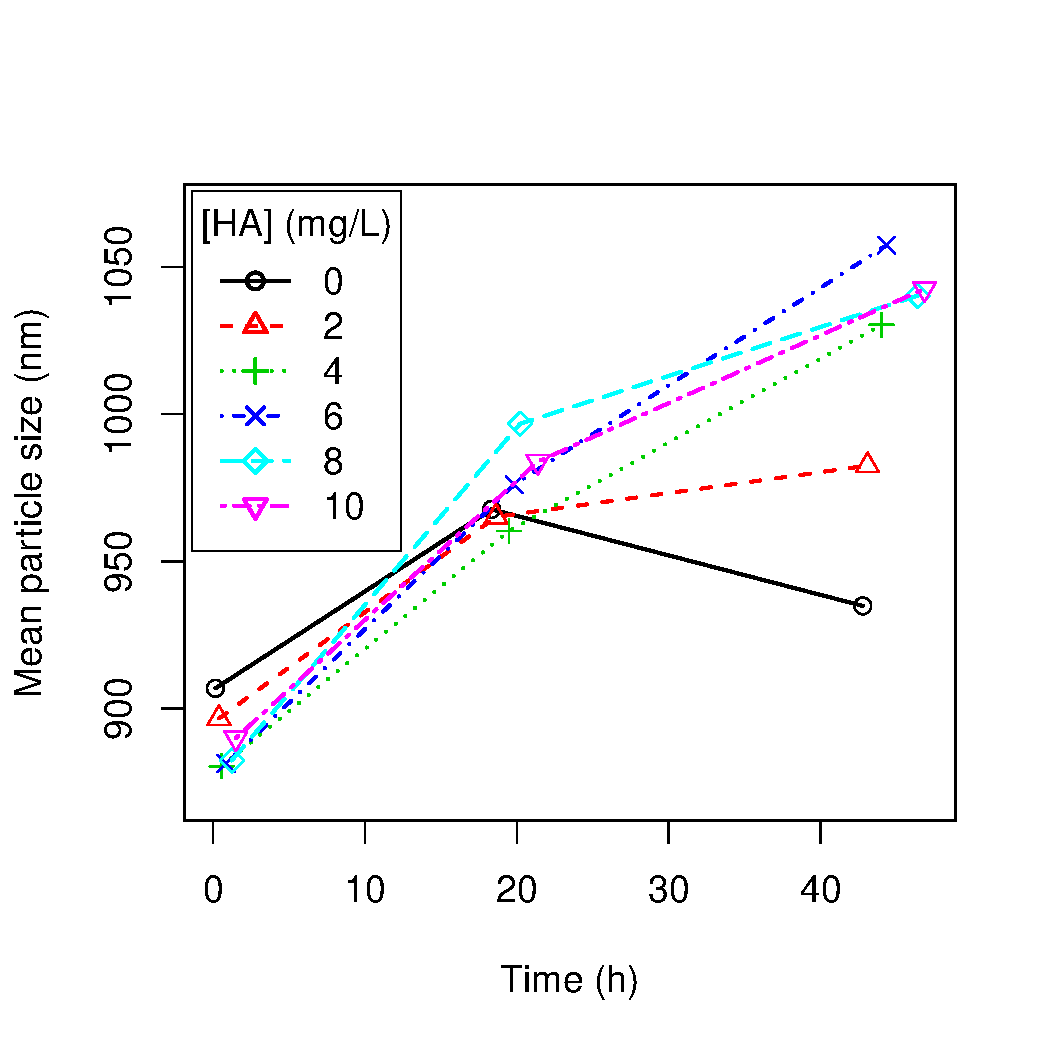
\includegraphics[width=\linewidth]{Figures/mean_particle_size.pdf}
  \caption{Time course of the evolution of the particle size, calculated by the  ratio moment 4 divided by the moment 3, for different concentrations of humic acids.} 
  \label{fgr:meansize}
\end{figure}
%% =========================================================================



% En esta parte solamente describimos los resultados, no aventuramos ninguna 
%  ya sabemos que los HA en CaCl2 NO producen Blockades (apenas) :-)!!!!


%Gaussian finite mixture model fitted by EM algorithm   

The optimal  kernel density function was in general fitted with a mixture of three gaussian components with different variances.
In one case,
$0.25~\mathrm{h}$
$\mathrm{[HA]\, = 6\, mg\,L^{-1}}$ had four components. The density histograms and best fitting  kernel density plots,
Figure~\ref{fgr:multiplot_density},
give an overview  of the changes in the particle size distribution by influence of the 
incubation time and the [HA]. 
Details of the distribution of the particles in  individual components or clusters is commented in the following subsections.

%%========================================================================= 
 \begin{figure}
  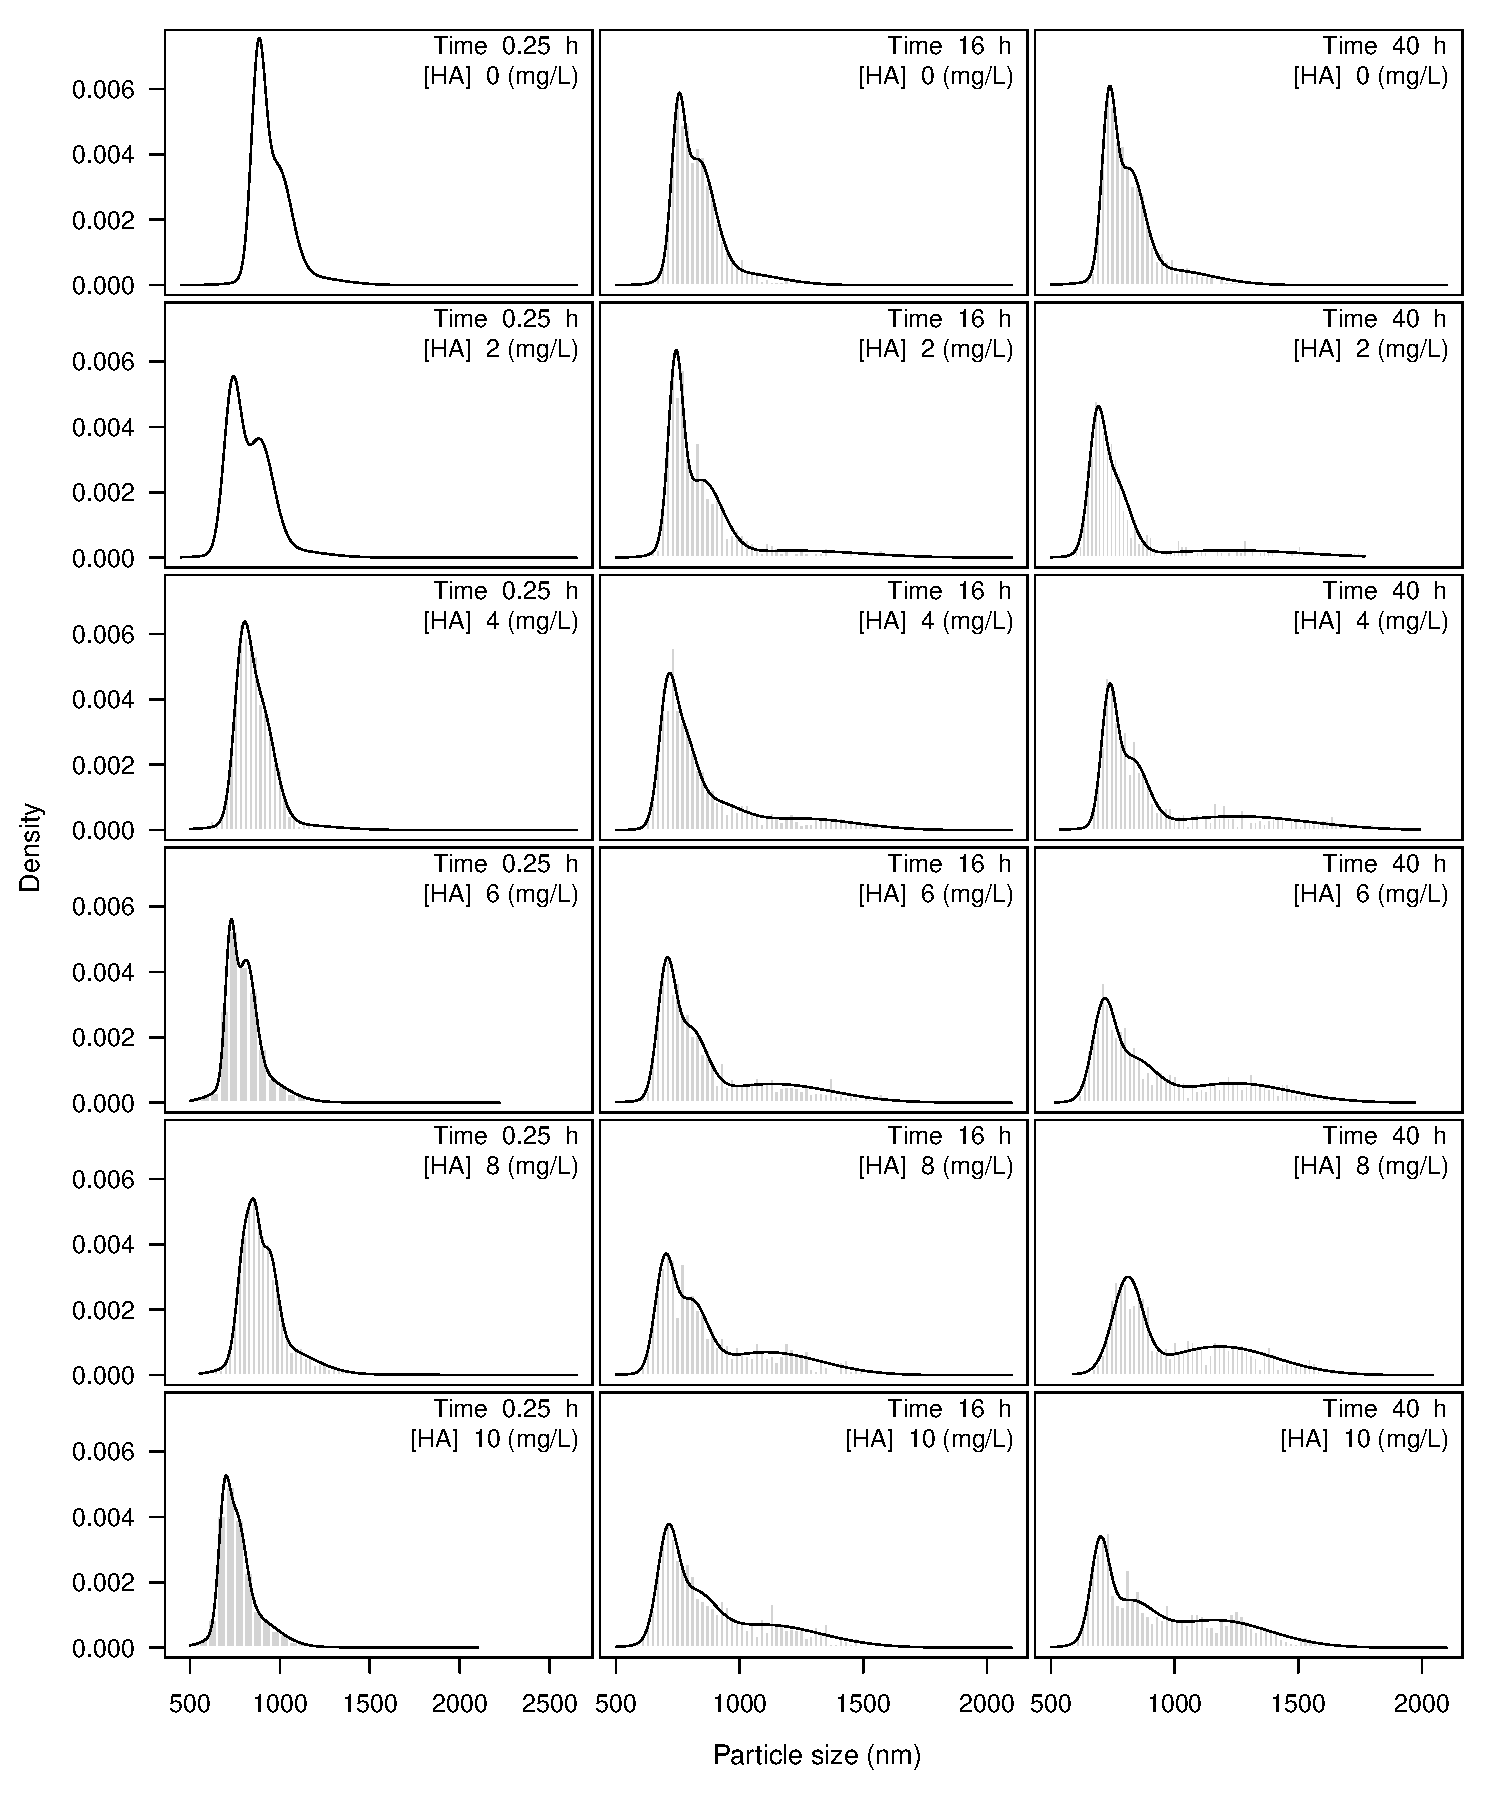
\includegraphics[width=\linewidth]{Figures/MCluster_MS_HA_density.pdf}
  \caption{Histograms and best fitting kernel density function (line) describing the influence of incubation time and the concentration of humic acids on the particle size distribution determined by tunable resistive pulse scanning. Plots show multiple components and density shifts to larger sizes with increasing the concentration of humic acids and incubation time. The number of blockades in each measurement was greater than $5000$.} 
  \label{fgr:multiplot_density}
\end{figure}
%% =========================================================================

\begin{table}
\label{tbl:sizes}
\caption{Mean and variance of particle diameter measured by TRPS that correspond to the best fitting gaussians obtained from the EM clustering algorithm. Values are displayed for each of the [HA] and contact times of MS and HA in \ce{CaCl2}.}
\begin{tabular}{r r rr rr rr}
[HA] &Time &
mean  & var.  &
mean  & var.  &
mean  & var.  \\
\hline
& & \multicolumn{2}{c}{Cluster 1}&
\multicolumn{2}{c}{Cluster 2}&
\multicolumn{2}{c}{Cluster 3} \\
\hline  
 0 & 0.25 & 713 & 991 & 787 & 4543 & 866 & 31755 \\ 
 0 & 16 & 969 & 1852 & 909 & 207 & 1069 & 60279 \\ 
 0 & 40 & 731 & 855 & 813 & 3000 & 959 & 27462 \\ 
 2 & 0.25 & 709 & 1037 & 798 & 3627 & 841 & 22213 \\ 
 2 & 16 & 762 & 2053 & 882 & 11813 & 1453 & 51244 \\ 
 2 & 40 & 737 & 1712 & 838 & 8097 & 1461& 52821 \\ 
 6 & 0.25 & 711 & 1087 & 796 & 2908 & 896 & 49951 \\ 
 6 & 16 & 700 & 639 & 776 & 4396 & 1120 & 66499 \\ 
 6 & 40 & 754 & 3051 & 872 & 13321 & 1393 & 50979 \\ 
 6 & 0.25 & 698 & 1303 & 782 & 4260 & 921 & 47950 \\ 
 6 & 16 & 704 & 985 & 794 & 4215 & 1078 & 56600 \\ 
 6 & 40 & 721 & 2122 & 830 & 12745 & 1272 & 71453 \\ 
 8 & 0.25 & 695 & 632 & 779 & 4667 & 903 & 32813 \\ 
 8 & 16 & 698 & 1299 & 797 & 5097 & 1112 & 52125 \\ 
 8 & 40 & 707 & 2561 & 806 & 6201 & 1119 & 55612 \\ 
 10 & 0.25 & 703 & 1341 & 789 & 8548 & 981 & 63088 \\ 
 10 & 16 & 702 & 1336 & 810 & 3700 & 1057 & 49303 \\ 
 10 & 40 & 729 & 3537 & 982 & 17527 & 1200 & 45689 \\ 
\hline
\multicolumn{8}{l}{[HA] in $\mathrm{mg\,L^{-1}}$; Time in $\mathrm{h}$; mean and variance (var.) in $\mathrm{nm}$.} 
\end{tabular}
\end{table}


%=========================================================================

Figure~\ref{fgr:boxplot_size} figure  shows the results of the particle size decomposition in three
different clusters. Note that particle size in the cluster no.~1 is smaller than the nominal particle size provided by the supplier. This is because this nominal size was used as reference size for calibration.  
%revisar esto
The cluster no.~2 is on the particle size reported by the manufacturer and the cluster no.~3 is above.
That indicates that TRPS
detects polydispersivity of the MS standards at early times, {\em i.e.} 5 min, in presence of \ce{CaCl2} and in absence of HA.


%% Cluster numero 1 azul 
The cluster no.~1 groups the particles in the range from $700$ to $810\;\mathrm{nm}$
the size of particles in the cluster no.~1 not varied upon the incubation time and the HA concentration. That means that there is a significant population of MS which size was not influenced by the HAs.
The largest deviations in the PSD corresponded to the absence of HA and the smaller concentration, 
$\mathrm{[HA]  < 2\,mg\;L^{-1}}$.
%Recall that 
%$\mathrm{[HA] =\; 2\; mg\,L^{-1}}$
%was about 30~times the stoichometric rate required for  coating the MS with a monolayer of HA.
This is because the separation between clusters at low [HA] or early times is not well defined. For example, in absence of HA at $24~\mathrm{h}$ incubation the populations assigned to clusters 1 and 2 are very close one to other. On the contrary, with larger HA concentrations and long  times cluster separation is neat.


%% Cluster numero 2 verde 
The cluster no.~2 groups the particles with size in the range from $800$ to $980\;\mathrm{nm}$.
Clusters no.~1 and 2 no not overlap except some extreme values with [HA]$\leq\, 2\;\mathrm{mg\,L^{-1}}$. At times $0 - 24~\mathrm{h}$ and
[HA] in the range $4 - 6~\mathrm{mg\, L^{-1}}$ the variance of PSD decreased, and the size regarding the smaller [HA].
Large variance  and sizes at low [HA] and time $< 24~\mathrm{h}$ is an ''statistical artifact'' that results from the lack of clear separation of the particle size components. So that it not represent a true population.
There is an increase of the particle size in the interval
of [AH] $4-10~\mathrm{mg\,L^{-1}}$.
The rate of increase in diameter with the [HA] was
$4.6\,\pm 1.8~\mathrm{nm\,L\,mg^{-1}}$, with a $\mathrm{P = 0.027}$ $r^2 > 0.635$ and 11 degrees of freedom. 
That confirms, that the size of particles in the cluster no. 2 increases significantly with the [HA] and the growth rate manifests at $24~\mathrm{h}$ incubation.

% Pendiente de Realizar puebas estadisticas del modelo lineal (tamaño ~[HA])


%%Cluster numero 3 rojo.
Cluster no. 3 groups the particles with the largest size
($> 980~\mathrm{nm}$). 
 At short times, 
$0.25~\mathrm{h}$,
there was a monotonic increase in size with the [HA] in the range
$2-8~\mathrm{mg\,L^{-1}}$.
At larger contact times, 
$24-48~\mathrm{h}$, 
the size increased dramatically 
with a maximum at $\mathrm{[HA]} = 2~\mathrm{mg\,L^{-1}}$ .
Then, at higher [HA] the size  decreases with a
monotonic decrease that can be clearly observed at 
$48~\mathrm{h}$.
The higest size, $1462~\mathrm{nm}$,
occurred
with
$\mathrm{[HA]} = 2~\mathrm{mg\,L^{-1}}
$ at 
$48~\mathrm{h}$.
This maximum size is equivalent to double the size of particles in the cluster no. 1, indicating that that this size may correspond to MS aggregates. %Laura: comprobar con microscopía, tenemos fotos?

%%========================================================================= 
 \begin{figure}
  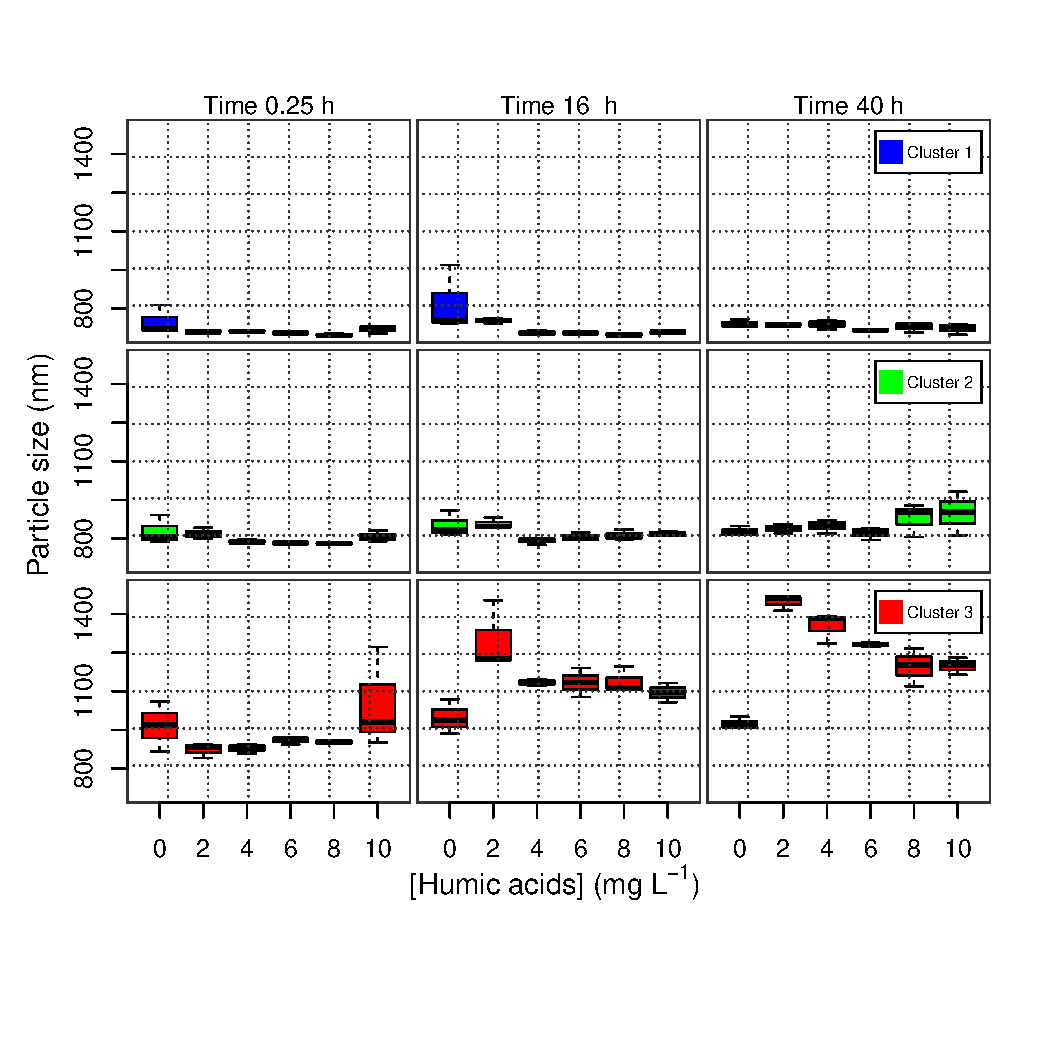
\includegraphics[width=\linewidth]{Figures/Boxplot_MS_HA_CaCl2_sizes.pdf}
  \caption{Influence of the concentration of Humic Acids and HA-MS contact time on the  size of MS.  Clusters numbered from 1 to 3 correspond to three gaussians that were identified by optimal fitting using the EM algorithm  that minimizes the BIC. The incubation times of the MS,  namely 0.25, 24 and 48, are indicated by labels on the top of the panels.}
  \label{fgr:boxplot_size}
\end{figure}
%%======================================================================== 





%%=========================================================================
\subsection{Distribution of particle populations}
% En esta parte solamente describimos los resultados, no aventuramos ninguna 
% hipótesis porque no sabemos que es lo que ocurre realmente.
% Puede ocurrir que e  el cluster 1 solamente existan MS, y en los demás
% clusters solamente existan HA floculados.
% Así que estamos a la espera de los resultados de Laura.

Classification of particles in different sizes was used to analyze the changes in the population distribution in function of time and [HA].
Figure~\ref{fgr:boxplot_populations} shows the distribution of populations,
namely, the fraction of particle counts in each size fraction frequencies 
regarding the influence of [HA].

%Analisis de las poblaciones en el Cluster 1 azul
Populations in the smaller cluster no .1 constitute less than the half of total TRPS counts.  Do not show a clear relation with the [HA] and 
time. 
Only  shows a  significant decrease 
with the [AH] in the range $2-6~\mathrm{mg\,L^{-1}}$ 
at 
$48~\mathrm{h}$ that can be related with the increase of the larger particles in the cluster no. 3 in the same 

%Analisis de las poblaciones en el Cluster 2 verde
Cluster 2
%($900 - 980~\mathrm{nm}$)
had the highest counts, i.e.
$>\,0.5$ population fraction, 
 at short times
,$0.25~\mathrm{h}$,
with a significant decrease at the maximum [HA], 
$10~\mathrm{mg\,L^{-1}}$.
At larger times the population decreased significantly in the range
of [AH] $2-8~\mathrm{mg\,L^{-1}}$.
Changes in the particle populations in the cluster no. 2 do not have
significant correspondence  with changes populations in the cluster no. 1.
Only  the  significant decrease  occurred
with [AH] $2-6~\mathrm{mg\,L^{-1}}$ 
at 
$48~\mathrm{h}$.






%Analisis de las poblaciones en el Cluster 3 rojo
In Cluster 3 
%($ > 980~\mathrm{nm}$)
populations varied in a opposite way as in the cluster no. 2. Figure~\ref{fgr:boxplot_populations}
shows a clear increase in numbers with the [HA] and contact time.
This increase corresponds to a decrease in the particle counts in the cluster no. 2.
%
% Lo que ocurre con 2 mg/L HA (cross linking)
That increase of in size regarding [HA] is not strictly monotonic.
 At concentrations 
$\mathrm{[HA]} = 2~\mathrm{mg\,L^{-1}}$ 
the  population reached the  minima, $0.12$ and $0.15$ of the total population. These particles correspond
with the largest sizes, doubling the diameter of the primary MS,  
$1300~\mathrm{nm}$ at
$24~\mathrm{h}$ 
and
$1462~\mathrm{nm}$ at
$48~\mathrm{h}$. 
That decrease agree with the flocculation behavior at 
$\mathrm{[HA]} = 2~\mathrm{mg\,L^{-1}}$ 
discussed above.



%===========================================================================
\begin{figure}
 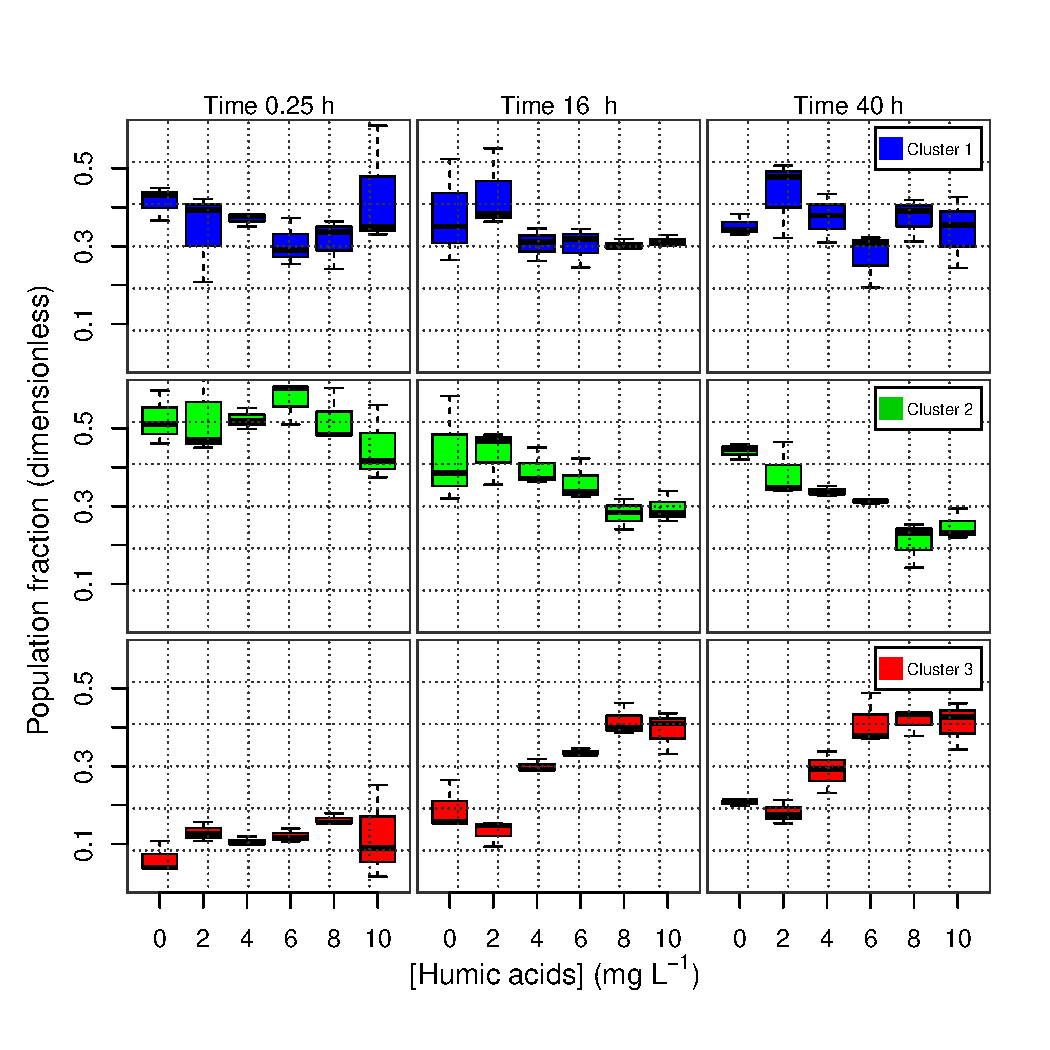
\includegraphics[width=\linewidth]{Figures/Boxplot_MS_HA_CaCl2_populations.pdf}
  \caption{Influence of the Humic Acids concentration and HA-MS contact time on the population distribution of MS into three particle size fractions denoted as
  Cluster 1 ($700 - 810~\mathrm{nm}$),  Cluster 2 ($900 - 980~\mathrm{nm}$), 
  and
  Cluster 3 ($ > 980~\mathrm{nm}$)
  }
  \label{fgr:boxplot_populations}
\end{figure}
%===========================================================================





%%=====================================================================
%%Discussion
%%=====================================================================

\section{Discussion}


%
The suitabiliy of TRPS to study colloid particle sizes
can be limited by the \ce{pH} and ionic strength  values that  control the flocculation rate.
Fortunately, the optimal pH and \ce{[Ca^{2+}]} for the TRPS measurements fall into the
typical values of the
soil solution\cite{wolt1994soil}
and  fresh water environments\cite{Stumm1993}.
Therefore, TRPS can be used to characterize the colloidal suspensions in a wide span of these of  aquatic samples and soils.

%Discusión: floculacion excesiva por elevada fuerza iónica
Large aggregates exceeding  the size of 
the measurement pore in the TRPS cannot be measured.

% Aqui discutimos la parte de la \subsection{Clustering particle sizes}

From these observations it can be drawn some findings  about the HA-MS interactions in presence of \ce{Ca^{2+}}.
First consider that the reference standards MS is not a single unimodal population.
%Laura: pedirle los  datos de las cuentas de calibración para comprobar mediante clustering si la distribución es unimodal o no
TRPS and clustering confirms reported using flow cytometry that the population can be optimally described by three gaussians.
 For example the  high resolution DLS procedure suggested by
 ~\citeauthor{Bryant2003AccurateSuspensions}\cite{Bryant2003AccurateSuspensions} 
reported  that poly(methyl methacrylate)-based particles have negatively
skewed particle size distributions and in many cases could be characterized
by the Weibull extreme value distribution. This type of distribution also
was found by fitting the overall particle size distribution obtained by TRPS. However, statistical clustering on TRPS data can resolve different components.


% Comparar métodos con los resultados que tenemos con citometria de flujo: Buscar las figuras de citometría de los resultados de Almudena.
%%
Second, there is a fraction of MS (Figure~\ref{fgr:boxplot_populations})
that is not influenced by the presence of HA, even in presence of \ce{CaCl2}
and HA at concentrations several times higher than level for complete
covering of the MS surface.
%%
Third, the intermediate component (cluster no. 2) clearly indicates  an
increase in particle size associated with the [HA] and
contact time. The coexistence of different sizes and the
slow  growth rate indicate that the kinetics of HA binding
to MS is slow. Adsorption of HA on PS MS is limited by
transport and electrostatic interactions~ \cite{doi:10.1021/es981236u}.
Double layer interaction calculations (Table~\ref{tbl:dvlo_interaction}) show a small potential gradient  low  repulsion barrier,
so that the attraction force  is small  and range of electrostatic attraction is short $\sim 20~\mathrm{nm}$.
The rate of increase in size is about one  layer of primary particles of HA per $\mathrm{mg HA\,L^{-1}}$ in the suspension.

%%
Fourth, the dramatic increase in size in cluster no. 3 
and subsequent decrease indicates bridging flocculation at 
$\mathrm{[HA] \,=\, 2\;mg\,L^{-1}}$, followed by polymer stabilization at higher [HA]. %% Pendiente de confirmar por microscopía.
Bridging flocculation and polymer stabilization can occur in any colloid that can adsorb dissolved organic matter and in presence of \ce{Ca^{2+}}.

Transition from bridging flocculation to polymer stabilization results from the stoichometry ratio of 
\ce{Ca^{2+}}:HA.
With 
$\mathrm{[HA]} = 2~\mathrm{mg\,L^{-1}}$ there is enough 
\ce{Ca^{2+}} to stabilize HA-MS bindings. However, at higher concentrations
the most
\ce{Ca^{2+}}
can be  complexed by the excess of HA  so that little
\ce{Ca^{2+}}
is available to strength the polymer bridges between ms.
The overall mechanism  result in a slow thickening of the MS coating. 

















 










\section{Conclusions}



TRPS provides a very good resolution in the separation  of particle sizes in polydisperse mixtures.



Alternative techniques to study surface adsorption such as laser-beam reflectometry.

That separation must be accompanied by a careful statistical statistical clustering procedure.

The quality of reparation depends on the neatness definition of subpopulations. A continuous broad distribution of particle sizes cannot bring an statistical separation.

The linear relationship  between particle size growth and [HA] sketches new potential methods based on TRPS to
quantify the influence of coating of MS by HA on the thickening of particles.

%=========================================================================
Results   a new approach to a more precise knowledge of the role of dissolved
organic polymers on the colloid behavior of particles  in soil and porous media in general. Constitute a contribution in fields related to 
water quality, environment and public health.
%=========================================================================



%%%%%%%%%%%%%%%%%%%%%%%%%%%%%%%%%%%%%%%%%%%%%%%%%%%%%%%%%%%%%%%%%%%%%
%% The "Acknowledgement" section can be given in all manuscript
%% classes.  This should be given within the "acknowledgement"
%% environment, which will make the correct section or running title.
%%%%%%%%%%%%%%%%%%%%%%%%%%%%%%%%%%%%%%%%%%%%%%%%%%%%%%%%%%%%%%%%%%%%%
\begin{acknowledgement}

%The authors thanks 
%Camille Roesch, Izon Europe Ltd. for technical supporting the TRPS.
This
work is partially funded by an AA1-GRC research contract (UE-FEDER,
Xunta de Galicia GRC2014/017), Diego-Soto by Spanish Government MEC’s FPU.

\end{acknowledgement}

%%%%%%%%%%%%%%%%%%%%%%%%%%%%%%%%%%%%%%%%%%%%%%%%%%%%%%%%%%%%%%%%%%%%%
% The same is true for Supporting Information, which should use the
%% suppinfo environment.
%%%%%%%%%%%%%%%%%%%%%%%%%%%%%%%%%%%%%%%%%%%%%%%%%%%%%%%%%%%%%%%%%%%%%
\begin{suppinfo}

This will usually read something like: ``Experimental procedures and
characterization data for all new compounds. The class will
automatically add a sentence pointing to the information on-line:

\end{suppinfo}

%%%%%%%%%%%%%%%%%%%%%%%%%%%%%%%%%%%%%%%%%%%%%%%%%%%%%%%%%%%%%%%%%%%%%
%% The appropriate \bibliography command should be placed here.
%% Notice that the class file automatically sets \bibliographystyle
%% and also names the section correctly.
%%%%%%%%%%%%%%%%%%%%%%%%%%%%%%%%%%%%%%%%%%%%%%%%%%%%%%%%%%%%%%%%%%%%%
\bibliography{Mendeley,Laura}

\end{document}


%% MANUAL DE USO


%New float types are automatically set up by the class file.  The
%means graphics are included as follows (Scheme~\ref{sch:example}).  As
%illustrated, the float is ``here'' if possible.
%\begin{scheme}
%  Your scheme graphic would go here: \texttt{.eps} format\\
%  for \LaTeX\, or \texttt{.pdf} (or \texttt{.png}) for pdf\LaTeX\\
%  \textsc{ChemDraw} files are best saved as \texttt{.eps} files:\\
%  these can be scaled without loss of quality, and can be\\
%  converted to \texttt{.pdf} files easily using \texttt{eps2pdf}.\\
%  %\includegraphics{graphic}
%  \caption{An example scheme}
%  \label{sch:example}
%\end{scheme}

%Adding notes to tables can be complicated.  Perhaps the easiest
%method is to generate these using the basic
%\texttt{\textbackslash textsuperscript} and
%\texttt{\textbackslash emph} macros, as illustrated %(Table~\ref{tbl:notes}).
%\begin{table}
%  \caption{A table with notes}
%  \label{tbl:notes}
%  \begin{tabular}{ll}
%    \hline
%    Header one                            & Header two \\
%    \hline
%    Entry one\textsuperscript{\emph{a}}   & Entry two  \\
%    Entry three\textsuperscript{\emph{b}} & Entry four \\
%    \hline
%  \end{tabular}
 % \textsuperscript{\emph{a}} Some text;
 % \textsuperscript{\emph{b}} Some more text.
%\end{table}